Muons are identified as the top priority in the reconstructed object list.
Besides the globale fit results, a constraint of 3 standard deviation of uncertainty should be satisfied between the momentum of the two tracks.
The tracks are then masked from the ingredient list along with a small subtraction of the expected energy deposits of muons passing through the ECAL (around 3 \GeV) and HCAL (around 0.5 \GeV) system from the clusters laying on the muon trajectory.
The following section will introudce the muon reconstruction and identification in the CMS experiment.

\subsection{Muon reconstruction}
The muon reconstruction is based on track reconstruction since muons leave energy deposits as hits in all subdetectors.
The muon reconstruction in the CMS experiment can be categorized into three different ways:

\begin{itemize}
    \item Standalone muon is reconstructed using hit information from the CSC, DT, and RPC in the muon detector.
        The process begins with track seeding with the DT or CSC segments and then iterate with the KF technique to build the muon tracks.
    \item Tracker muon is made by extrapolating the tracks, with $\PT > 0.5 \GeV$ and a total momentum $p > 2.5 \GeV$, in the tracker system to the muon system with loosely mathcing to the DT or CSC segments.
        The inner track is considered as a tracker muon track if at least one muon segment matching with the extrapolated track.
    \item Global muon is built by comparing the tracks from standalone muon with tracker system.
        A combined fit is performed by the KF technique to construct a global muon track with information of both the standalone muon tracks and tracks from tracker system, if the parameters of those tracks are matched .
\end{itemize}

Thanks to the high efficiency of the tracker system and muon segment reconstruction, about $99\%$ muons received in the detector acceptance can be successfully reconstructed as tracker muons and global muons,
The tracks can be further merged as a single object if the global muon tracks match to the track muon track.
The associated PF ingredients are then removed from the ingredient list once the muons are reconstructed.

The momentum measurement of muon is performed with a Tun-P algorithm to obtain the precise momentum of muon in different situations.
The algorithm of \PT measurement can be separated into 4 kinds by goodness-of-fit and $\sigma(\PT)/\PT$ criteria:

\begin{itemize}
    \item Inner-track fit uses the information only from the tracker system to determine the momentum.
        The Tune-P algorithm prefers this method for low \PT muons, since the muon detector has less contribution for momentum reconstruction for muons with $\PT < 200 \GeV$.
    \item Tracker-Plus-First-Muon-Station (TPFMS) fit performs a refit to the hits of the global muon track from the tracker system and muon detectors, since the innermost muon detectors give the best muon momentum information among the muon detectors.
    \item Picky fit also takes the hits from the global muon track like TPFMS fit.
        However, it focuses on large hit occupancy such as a shower taking place in the muon chambers.
        In this case, only hits compatible to the extrapolated trajectory based on $\chi^2$ are added into the refit work.
    \item Dynamic-Truncation fit focuses on the case that significantly bent muon trajectory caused by energy loss.
        This method performs a refit with the inner-track extrapolated to the innermost muon detectors and added compatible hits from the segment closest to the extrapolated trajectory.
\end{itemize}

\subsection{Muon identification and isolation}
Muons leave a clear path in both the inner tracking system and muon detectors outside the solenoid.
This iconic signature of muon can be used to determine a great deal of information of the reconstructed muon properties.
The track provides sufficient information in the tracking system with itself being a good fit of the hits and with minimal amounts of invalid hits along the track.

In this analysis, we focus on muons originating directly from a hard scattering process instead of muons coming from secondary decay products of short-lived hadrons.
Therefore, the muon track should be with a primary vertex and occupy all inner tracker system, rather than just a segment.

The muon physics object group defines standard selection criteria for different levels of muon identification (ID) depending on the analysis needs~\cite{CMS:mu_PF}.
A tight muon is required to meet the following criteria:
\begin{itemize}
    \item The candidate is reconstructed as a Global Muon with tracks fitting starting from the muon subdetectors.
   \item Identified by the particle flow algorithm as a muon 
    \item The $\chi^2$/d.o.f of the track fitting should be smaller than 10, at least one muon chamber hit included in the global muon track fit, and muon segments in at least two muon stations.
        These selections suppress hadronic punch-through and muons from decays in flight, that is, suppress accidental track-segment matching, where the inner track might be generated from a particle other than the muon.
    \item The corresponding track having a transverse impact parameter with the primary vertex $d_{xy} < 2$ mm, and a longitudinal distance $d_z < 5$ mm.
        This cut suppress cosmic muons and further suppress muons from decays in flight, while preserves muons originating from the semi-short-lived \PQb and \PQc hadrons.
    \item At least one pixel hit to suppress muons from hadrons decaying in flight.
    \item More than 5 tracker layers hit to guarantee a good \PT measurement.
\end{itemize}

A loose muon, on the other hand, is only required to meet the following criteria:
\begin{itemize}
    \item The candidate is reconstructed as a Global Muon with tracks fitting starting from the muon subdetectors or reconstructed as a track muon.
    \item Identified by the particle flow algorithm as a muon 
\end{itemize}

In order to distinguish prompt muons from the \PW and \PZ bosons decay against those from heavy flavor decays within jets, a particle flow based relative isolation value, noted as $I_{\mathrm{pf,rel}}$, is computed by comparing the momentum of the muon track with the energy deposits in adjacent subsystems~\cite{CMS:mu_PF} and defined as
\begin{linenomath}\begin{equation}\label{eq:reco_muon_iso}
    I_{\mathrm{pf,rel}} = \frac{ \sum p_{\mathrm{T,chhad}} + \mathrm{max}(0, \sum E_{\mathrm{T,neuhad}}  +   \sum E_{\mathrm{T,}\gamma} -  0.5\sum p_{\mathrm{T,pileup}})     }{  p_{\mathrm{T,}\mu} }
\end{equation}\end{linenomath}
where the various $\sum p_{\mathrm{T,x}}$s are the sum of the transverse momentum (or energy) of the charged hadrons, neutral hadrons, photons, and pileup energy within an angular separation $\Delta R < 0.4$ around the muon, and $p_{\mathrm{,\mu}}$ is the transverse momentum of the muon itself.
Designated working points of cut on the $I_{\mathrm{pf,rel}}$ is determined by the muon physics object group.
This analysis choose a tight working point $I_{\mathrm{pf,rel}} < 0.15$ and tight working point ID, giving more than $96\%$ efficiency as shown in Fig.~\ref{fig:reco_muon_eff}.

\begin{figure}\centering
    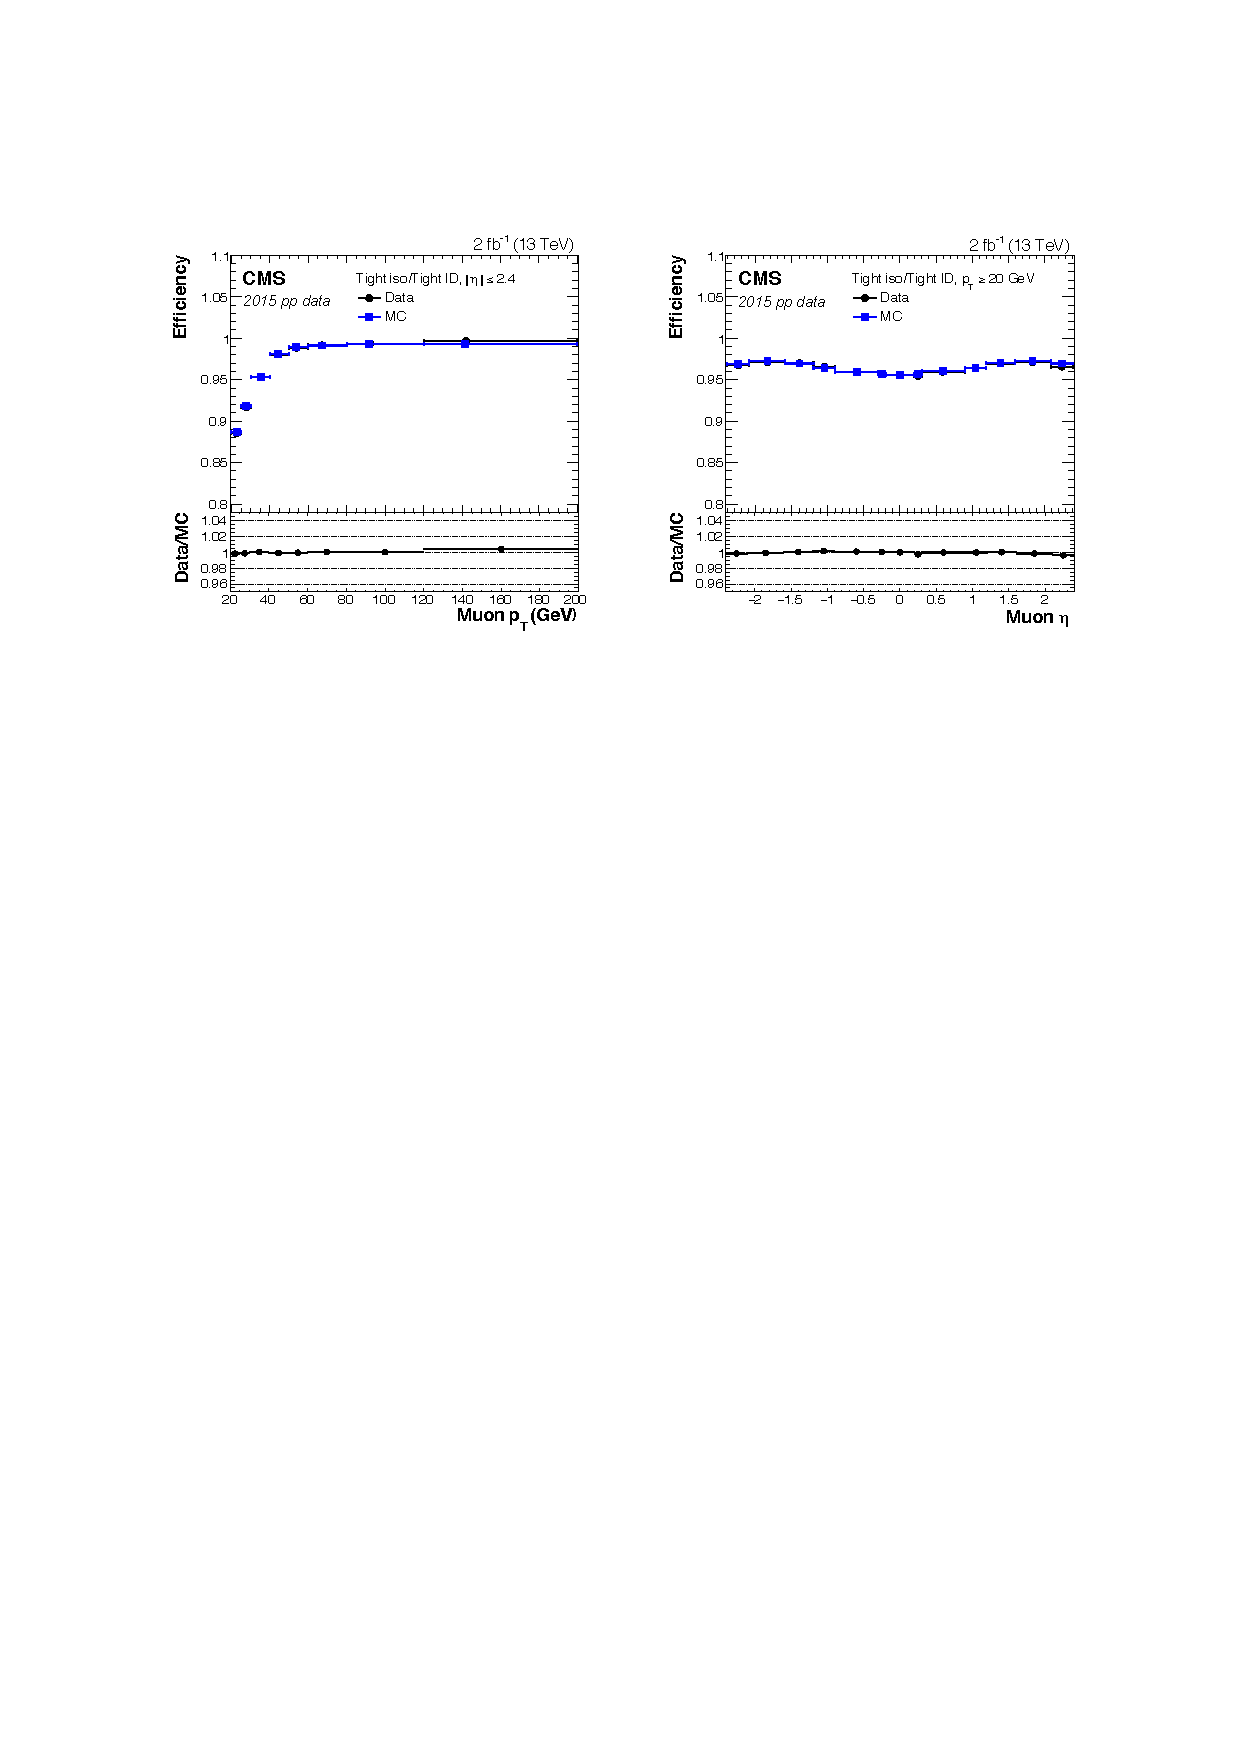
\includegraphics[width=\textwidth]{figure/reco_muon_eff.pdf}
    \caption[Tag-and-probe muon efficiency for the tight PF isolation working point on top of the tight ID]{
        Tag-and-probe efficiency for the tight PF isolation working point on top of the tight ID versus \PT for muons in the acceptance of the muon spectrometer (left), and versus $\eta$ for muons with $\PT > 20 \GeV$ (right), for 2015 data (circles), simulation (squares), and the ratio (bottom inset).
        The statistical uncertainties are smaller than the symbols used to display the measurements.
    }
    \label{fig:reco_muon_eff}
\end{figure}


